\documentclass[a4j,10pt,uplatex]{jsarticle}

\usepackage[top=30mm, hmargin=20mm, bottom=25mm]{geometry}
\usepackage{ipsj}
\usepackage[dvipdfmx]{graphicx}
% \usepackage[dvipdfmx]{color}
% \usepackage{float}
%\usepackage{wrapfig}
\usepackage{amsmath, amssymb}
\usepackage{amsfonts}
% \usepackage{algorithm}
% \usepackage{algorithmic}
% \usepackage{theorem}
%\usepackage{ulem}
% \usepackage{bld}
%\usepackage{comment}
\usepackage{bm}
% \usepackage[table,xcdraw]{xcolor}
\usepackage[hang,flushmargin]{footmisc}
\usepackage{siunitx}
\sisetup{%
mode = text
}

\renewcommand{\baselinestretch}{0.85}

\graphicspath{{./fig/}}

\renewcommand\thefootnote{*\arabic{footnote}}

\makeatletter
\def\blfootnotetext{\xdef\@thefnmark{}\@footnotetext}

\renewenvironment{thebibliography}[1]
{\section*{\refname\@mkboth{\refname}{\refname}}%
  \list{\@biblabel{\@arabic\c@enumiv}}%
       {\settowidth\labelwidth{\@biblabel{#1}}%
        \leftmargin\labelwidth
        \advance\leftmargin\labelsep
 %\setlength\itemsep{-0.1zh}%←ここの数値を調整(行間のつまり具合)
 %\setlength\baselineskip{7pt}%←ここの数値を調整(追加)(文字の大きさ)
        \@openbib@code
        \usecounter{enumiv}%
        \let\p@enumiv\@empty
        \renewcommand\theenumiv{\@arabic\c@enumiv}}%
  \sloppy
  \clubpenalty4000
  \@clubpenalty\clubpenalty
  \widowpenalty4000%
  \sfcode`\.\@m}
 {\def\@noitemerr
   {\@latex@warning{Empty `thebibliography' environment}}%
  \endlist}
\makeatother

\parindent = 10pt
\setlength\textfloatsep{5pt}

% \newtheorem{theo}{定理}[section]
% \newtheorem{defi}{定義}[section]
% \newtheorem{lemm}{補題}[section]
% \theoremstyle{break}

\newcommand{\UAV}{{\rm UAV}}
\newcommand{\MA}{{\rm MA}}
\newcommand{\argmax}{\mathop{\rm argmax}\limits}

\jtitle{距離ベース時間周波数マスク推定による音声強調手法の検討}
\jcontact{$1$ 東京工業大学 工学院 システム制御系\quad $2$ (株) ホンダ・リサーチ・インスティチュート・ジャパン}
\jauthor{石井 遼平$^1$, 糸山 克寿$^1$, 中臺 一博$^{1, 2}$}

%本文
\begin{document}

\maketitle

\blfootnotetext{An Ensemble Method for Multiple Speech Enhancement Using Deep Learning}
\blfootnotetext{Ryohei Ishii$^1$, Katsutoshi Itoyama$^1$, Kazuhiro Nakadai$^{1, 2}$}
\blfootnotetext{$1$ Dept.~of Systems and Control Engineering, School of Engineering, Tokyo Institute of Technology\\
$2$ Honda Research Institute Japan Co., Ltd.}

\section{はじめに}
音声は意思疎通を図るうえで最も自然で使いやすい手段の一つである. 
コンピュータやロボットが実環境で音声を適切に扱うことができるようになれば, 
人との自然なコミュニケーションの実現に近づくことが期待される. 
ほとんどの場合, 実環境で収録された音声には雑音や残響が含まれており,
これらは音声認識などのサービスの性能を低下させてしまう.
音声強調は, 音声に混入した雑音や残響を取り除き,
人間にとって聞きやすく, コンピュータやロボットにとって処理しやすいクリーンな音声を得るための技術である.

音声強調はこれまでに数多く研究されている.
例えば, Heymannらはニューラルネットワーク (NN) を用いて時間周波数マスクを推定し, さらにこれをビームフォーミングと組み合わせる手法を提案した~\cite{Hey2016}.
時間周波数マスクは, 雑音混じり音声のスペクトログラムと同じサイズの行列として定義され, 
スペクトログラムとマスクの要素積をとることで目的音声のみを通過させ音源分離や音声強調を実現する手法である.
この手法には NN によってマスクを正確に推定できるという利点がある一方で, 
NN の学習に用いていない未知の環境雑音に対しては性能が劣化してしまうという問題がある.
この他にも, 独立成分分析 (ICA) \cite{comon1994independent} や非負値行列因子分解 (NMF) \cite{wilson2008speech} 等を用いた音声強調手法がこれまでに提案されているが, 
いずれの手法についても収録環境や雑音の種類に得手不得手があるため, 
あらゆる環境でロバストに動作する音声強調手法が必要とされている. 

本稿では, 畳み込みニューラルネットワーク (CNN) を用いて複数の音声強調処理をアンサンブルした,
環境や雑音の変化に対してロバストな音声強調手法を提案する.
アンサンブルは機械学習で用いられる識別器の汎化性能を向上させるために用いられる手法である.
複数の音声強調手法から生成された時間周波数マスクを CNN を用いてアンサンブルすることで, 
それぞれの手法の長所を併せ持つアンサンブル時間周波数マスクを生成し, 音声を強調する. 
% 入力音声ごとに適したマスクの生成が期待できる.

\section{提案手法}
\begin{figure}[t]
 \centering
 % 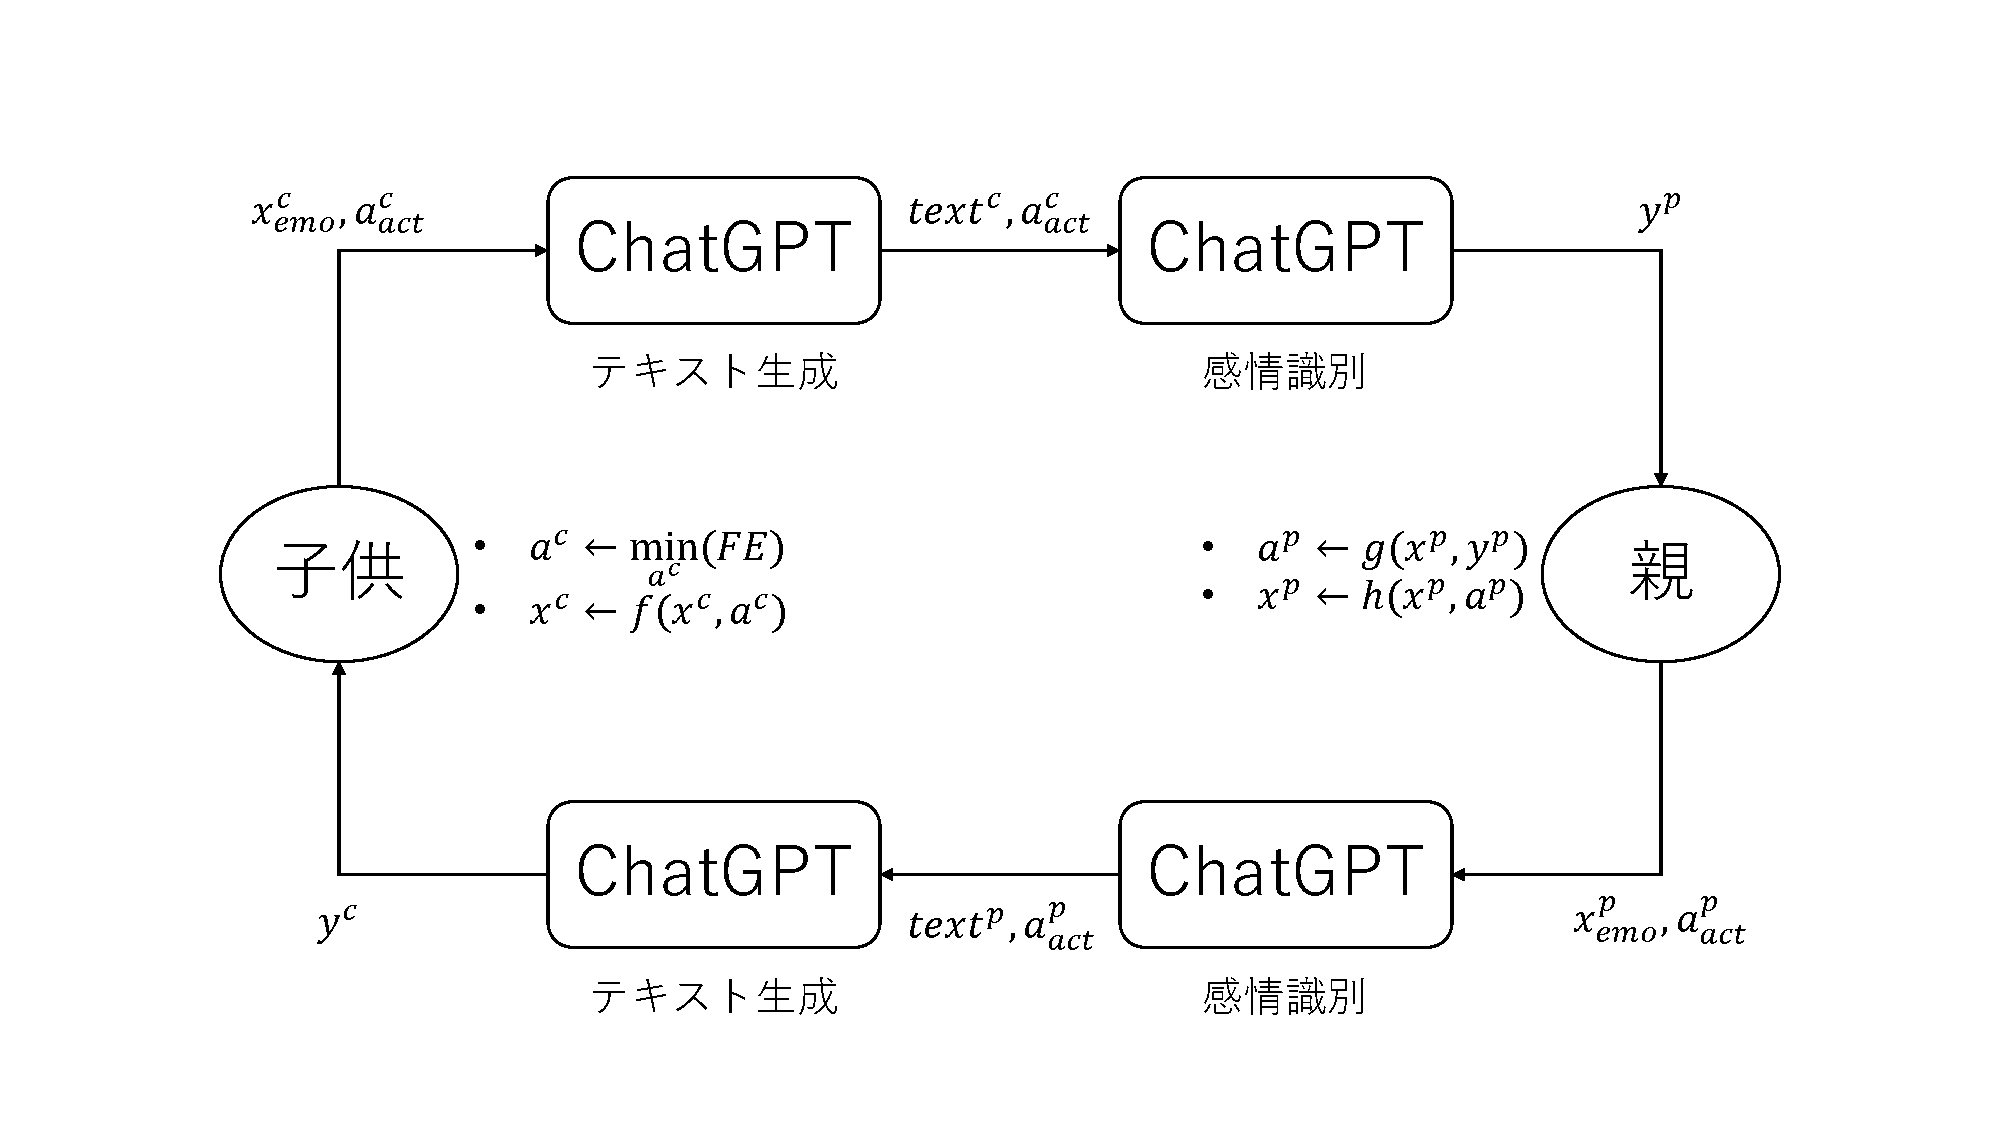
\includegraphics[width=1.\linewidth,pagebox=artbox]{./fig/system.pdf}
 \caption{提案手法のシステム概要} 
 \label{system}
\end{figure}
雑音を含む音声を入力として,
全$N$個の音声強調手法を用いてそれぞれで時間周波数マスクを推定する.
アンサンブルにより統合されたマスク(アンサンブル時間周波数マスク)を生成し,
これをもとにビームフォーミングを行い, 目的の音声を強調抽出する.
このシステムは藤田らが提案したもの
%\cite{fujita2021ipsj}
とほぼ同一の構成であるが,
マスクのアンサンブルに CNN を用いることで,  
時間周波数ごとに異なるマスク重みを入力音声に応じて推定することが可能となる. 
アンサンブル時間周波数マスクを用いたGeneralized EigenValue (GEV) ビームフォーミング~\cite{Hey2016} により,
最終的な強調音声を得る.
Fig.~\ref{system}に提案手法の概要を示す.

CNN の構成を Table 1 に示す.
\begin{table}[tbp]
\centering
\caption{CNN の構成} % letter
\begin{tabular}{c}
\hline
Input: $N$-ch time-frequency masks, $800 \times 512 \times N$ \\
\hline \hline
Conv2D $3 \times 3$ @ 32, ReLU \\
MaxPooling2D $2 \times 2$, $\text{stride} = 2$ \\
\hline
Conv2D $3 \times 3$ @ 16, ReLU \\
MaxPooling2D $2 \times 2$, $\text{stride} = 2$ \\
\hline
Conv2D $3 \times 3$ @ 8, ReLU \\
MaxPooling2D $2 \times 2$, $\text{stride} = 2$ \\
\hline
Conv2D $3 \times 3$ @ 8, ReLU \\
\hline
TransConv2D $2 \times 2$, $\text{stride} = 2$ @ 8, ReLU \\
\hline
TransConv2D $2 \times 2$, $\text{stride} = 2$ @ 16, ReLU \\
\hline
TransConv2D $2 \times 2$, $\text{stride} = 2$ @ 32, ReLU \\
\hline
TransConv2D $2 \times 2$, $\text{stride} = 2$ @ N, ReLU \\
\hline
Softmax \\
\hline
Multiply with input and sum \\
\hline \hline
Output: \qty{1}{ch} time-frequency mask, $800 \times 512$ \\
\hline
\end{tabular}

\end{table}
入力は各音声強調手法によって生成された $N$ch のマスクであり, 出力は $1$ch のアンサンブルマスクである.
全体の構成は, 2次元の畳み込みを行う前半部と逆畳み込みを行う後半部分に分かれる.
出力層の手前にソフトマックス関数を導入し, 入力との積を取ることで出力としている.
これは時間周波数マスクの各時間周波数ビンで次のような入力マスクの加重平均が
行われることを期待している.
\begin{eqnarray}
    \bm{\hat{M}}_{ft} = \sum_{n=1}^{N} \alpha_{nft} \bm{M}_{nft}
\end{eqnarray}
ここで, $\bm{\hat{M}} \in \mathbb{R}^{F \times T}$はアンサンブルマスク, 
$\bm{M}_{n} \in \mathbb{R}^{F \times T}$は各手法によって生成されたマスク, 
$\alpha_{n} \in \mathbb{R}^{F \times T}$は各マスクに対応する重み行列である.

\section{実験・考察}
提案手法の有効性を評価するために, シミュレーションによる実験を行った.
評価指標として Perceptual Evaluation of Speech Quality (PESQ)~\cite{PESQ} を用いた.
PESQは $-0.5$から$4.5$ までの実数値で表され, 
値が大きいほど人にとって聴きやすい音声であることを示す.

評価のためのデータセットをシミュレーションにより作成した.
クリーンな音声として CHiME3 dataset~\cite{barker2015third} 内の$4$話者の計$330$発話
(\qty{16}{\kilo\hertz}, \qty{16}{bit}, \qty{1}{ch}) を用いた.
雑音として, Freesound\footnote{https://freesound.org/}からダウンロードした
ヘリコプターの雑音 (Heli) とレストランの室内の雑音 (Babble) の 2 種類を用いた.
これらの雑音は \qty{44.1}{\kilo\hertz} で提供されているため
\qty{16}{\kilo\hertz} にダウンサンプリングした.
SN比が \qty{0}{\decibel} となるように音量を調節し,
Fig.~\ref{environment} に示すような環境で混合音を作成した.
\begin{figure}[t]
 \centering
 % \includegraphics[width=1.\linewidth,pagebox=artbox]{./fig/recording_situation.pdf}
 \caption{シミュレーション環境} 
 \label{environment}
\end{figure}
CNN の学習におけるオプティマイザには Adam を用い, 学習率は 0.001 とした.
損失関数として平均二乗誤差を用いた.

アンサンブルの対象の音声強調手法として次の 2 手法を用いた.
ひとつはNN でマスクを推定する手法 (NN)~\cite{Hey2016} である.
NN は CHiME3 dataset の学習用の模擬録音データによって学習されており, 
bus, cafe, pedestrian, street の 4 種類の雑音を既知としている.
%したがって, babble noise については既知の雑音ということになる.
もうひとつの手法として ILRMA~\cite{kitamura2016determined} を用いた.
ILRMA は低ランクな雑音の高精度な除去が可能である一方で, 
低ランクでない雑音を十分に取り除けない場合がある.
%よって, ILRMA による雑音処理において, heli noise は得意, babble noise は苦手
%ということが言える.

各音声強調手法で強調した音声を PESQ で評価した結果を Table 2 に示す.
Noisyは強調前の観測音声, NN, ILRMA, Proposedはそれぞれの手法による強調音声を表す. 
\begin{table}[t]
\caption{各手法により強調された音声のPESQスコア}
\begin{tabular}{c|c|c|c|c}
             & Noisy & NN   & ILRMA & Proposed      \\ \hline
Heli    & 1.12  & 2.08 & 2.72  & 2.27          \\ \hline
Babble  & 1.13  & 2.32 & 2.58  & \textbf{2.64} %\\ \hline
%All          & 1.13  & 2.22 & 2.63  & 2.49         
\end{tabular}
\end{table}
ILRMAは低ランクなHeliに対するPESQスコアが高く,
NNは既知であるBabbleに対するPESQスコアが高いことが分かる.
% Beli noise に対しては ILRMA が, Babble noise に対しては NN が優位に雑音除去ができている.
また, 提案手法は, Babble に対してNNとILRMAの強調性能を上回った.
この結果により, 提案手法は2手法の長所を併せ持つマスクを生成できることが示された. 
% これはアンサンブルによって 2 手法の良いところをうまく統合できたためだと考察する.

\section{おわりに}
CNN を用いた時間周波数マスクのアンサンブルを行う音声強調手法を提案した.
評価実験によって CNN によるアンサンブルの有効性を示した.

\paragraph{謝辞}
本研究はJSPS科研費 JP19K12017, JP19KK0260 および JP20H00475 の助成を受けた.

\footnotesize
\bibliographystyle{unsrt}   
\bibliography{cite}    % bibファイル名を指定する.拡張子は除く.

\end{document}
